\documentclass{ximera}

\newcommand{\RR}{\mathbb R}
\renewcommand{\d}{\,d}
\newcommand{\dd}[2][]{\frac{d #1}{d #2}}
\renewcommand{\l}{\ell}
\newcommand{\ddx}{\frac{d}{dx}}
\newcommand{\dfn}{\textbf}
\newcommand{\eval}[1]{\bigg[ #1 \bigg]}


\outcome{Compute volumes using the shell method.}
\outcome{Know when to use the shell method.}
\outcome{Set up integrals for the computing volume using the shell method.}

\title[Dig-In:]{Solids of revolution}

\begin{document}
\begin{abstract}
  We use the procedure of ``Slice, Approximate, Integrate" to compute volumes of solids with radial symmetry.
\end{abstract}
\maketitle


\section{Solids of revolution}\index{solid of revolution}
\index{volume of a solid of revolution}

Given a region $R$ in the $xy$-plane, we built solids by stacking ``slabs" with given cross sections on top of $R$.  Another way to generate a solid from the region $R$ is to revolve it about a vertical or horizontal axis of rotation.  A solid generated this way is often called a \emph{solid of revolution}. In this section, we study two methods used to compute the volume of such a solid.

Before we begin, we recall that in order to find the volume of a hollowed out cylinder with outer radius $R$, inner radius $r$, and height $h$:

\begin{image}
\begin{tikzpicture}

 	\draw (0,0) ellipse (1cm and .3cm);
	\draw (-1,0) -- (-1,1);
 	\draw (1,0) -- (1,1);
 	\draw (0,1) ellipse (1cm and .3cm);
 	\draw (0,1) ellipse (.6cm and .1cm);
   
\draw[penColor] (0,1) -- (1,1) node[anchor=north] { \qquad $R$};
\draw[penColor2] (0,1) -- (-.4,.92) node[anchor=south] {};
\draw[penColor2] (-.5,1.04) -- (-.5,1.04) node[anchor=north] { $r$};
\draw[penColor5] (-1.2,.7) -- (-1.2,.7) node[anchor=north] { $h$};
\end{tikzpicture}
\end{image}

\[
\textrm{Volume} = \pi R^2h-\pi r^2h=\pi(R^2-r^2)h 
\]
Note that the volume of a hollow cylinder requires only these geometric quantities of interest; it does not require that we work with a coordinate system!  However, in order to use calculus, we recognize that our solids of revolution will be formed by revolving regions in the $xy$-plane whose boundaries are functions of $x$ or $y$ about an axis of rotation.  Hence, one of the essential skills will be a familiar one; we must interpret the the inner and outer radii as well as the height in terms of our variable of integration!

\section{The Washer Method}

A solid of revolution is formed by revolving the region bounded $y=x^2-4$, $x=1$, and $y=5$ about the $y$-axis.  

 \begin{image}
            \begin{tikzpicture}
            	\begin{axis}[
            		domain=-10:10, ymax=6.8,xmax=3.4, ymin=-.8, xmin=-3.4,
            		axis lines =center, xlabel=$x$, ylabel=$y$,
            		every axis y label/.style={at=(current axis.above origin),anchor=south},
            		every axis x label/.style={at=(current axis.right of origin),anchor=west},
            		axis on top,
            		]
                      
            	\addplot [draw=penColor,domain=2:3,very thick,smooth] {x^2-4};
		\addplot [draw=penColor,domain=-3:-2,very thick,smooth] {x^2-4};
	         \addplot [draw=penColor2,very thick,dotted] coordinates {(1,0)(1,4.5)};
	          \addplot [draw=penColor2,very thick,dotted] coordinates {(-1,0)(-1,4.5)};
           	                            
            	%shades top
		\addplot [name path=A,domain=-3:3,draw=none,samples=200] {5+sqrt(.25- .25/9*x^2)};   
		\addplot [name path=B,domain=-3:3,draw=none,samples=200] {5-sqrt(.25- .25/9*x^2)};   
		\addplot [fillp!75] fill between[of=A and B];
		
		%shades outer part	
		\addplot [name path=C,domain=-3:3,draw=none,samples=200] {5-sqrt(.25- .25/9*x^2)};   
            	\addplot [name path=D,domain=-2:2,draw=none,samples=200] {-sqrt(.25- .25/4*x^2)};
	 	\addplot [name path=E,domain=2:3,draw=none] {x^2-4};
		\addplot [name path=F,domain=-3:-2,draw=none] {x^2-4};
	       	\addplot [fillp] fill between[of=C and D];
		\addplot [fillp] fill between[of=C and E];
		\addplot [fillp] fill between[of=C and F];
	     
                 %shades negative part	
                 \addplot [name path=G,domain=-3:3,draw=none,samples=200] {5+sqrt(.05- .05*x^2)};   
		\addplot [name path=H,domain=-3:3,draw=none,samples=200] {5-sqrt(.05- .05*x^2)};   
		\addplot [gray!20!fillp] fill between[of=G and H];
		\addplot [name path=I,domain=-1:1,draw=none,samples=200] {5-sqrt(.25- .25/9*x^2)};   
		\addplot [name path=J,domain=-1:1,draw=none,samples=200] {-sqrt(.05- .05*x^2)};   
		\addplot [gray!20!fillp] fill between[of=I and J];
		
                 %outer ellipses
                  \addplot [draw=penColor,domain=-3:3,very thick,smooth,samples=200] {5+sqrt(.25- .25/9*x^2)};
                  \addplot [draw=penColor,domain=-3:3,very thick,smooth,samples=200] {5-sqrt(.25- .25/9*x^2)};
                   \addplot [draw=penColor,domain=-2:2,very thick,smooth,samples=300,dashed] {sqrt(.25- .25/4*x^2)};
                  \addplot [draw=penColor,domain=-2:2,very thick,smooth,samples=300] {-sqrt(.25- .25/4*x^2)};
                  
                  %inner ellipses
                  \addplot [draw=penColor2,domain=-1:1,very thick,smooth,samples=200] {5+sqrt(.05- .05*x^2)};
                  \addplot [draw=penColor2,domain=-1:1,very thick,smooth,samples=200] {5-sqrt(.05- .05*x^2)};
                  \addplot [draw=penColor2,domain=-1:1,very thick,smooth,samples=200,dashed] {sqrt(.05- .05*x^2)};
                  \addplot [draw=penColor2,domain=-1:1,very thick,smooth,samples=200,dashed] {-sqrt(.05- .05*x^2)};
                  %%%%%%%%%%%%%%%%%%%%                 
            	\node at (axis cs:11,1.55) [penColor] {$x=4y^2$};
            	\node at (axis cs:15,-.9) [penColor2] {$x+4y=8$};
	    
	      \end{axis}
            \end{tikzpicture}
            \end{image}


How can we go about finding the volume of the resulting solid?  Let's try to apply the ``Slice, Approximate, Integrate" procedure.

\paragraph{Step 1: Slice}
The geometry of the base region suggests that it is advantageous to use horizontal slices.  This means we should:

\begin{multipleChoice}
\choice{integrate with respect to $x$.}
\choice[correct]{integrate with respect to $y$.}
\end{multipleChoice}

We indicate a prototypical slice of thickness $\Delta y$ at an unspecified $y$-value on the base:

 \begin{image}
            \begin{tikzpicture}
            	\begin{axis}[
            		domain=-10:10, ymax=6.8,xmax=4.2, ymin=-.8, xmin=-.8,
            		axis lines =center, xlabel=$x$, ylabel=$y$,
            		every axis y label/.style={at=(current axis.above origin),anchor=south},
            		every axis x label/.style={at=(current axis.right of origin),anchor=west},
            		axis on top,
            		]
                      
            	\addplot [draw=penColor,domain=0:9,very thick,smooth] {x^2-4};
	        \addplot [draw=penColor5,very thick,smooth] {5};
	        \addplot [draw=penColor2,very thick,smooth] coordinates {(1,-10)(1,10)};
            	\addplot [draw=penColor2,very thick,dashed] coordinates {(0,-10)(0,10)};
	                            
            	\addplot [name path=A,domain=1:3,draw=none,samples=200] {5};   
            	\addplot [name path=B,domain=1:2,draw=none,samples=200] {0};
	        \addplot [name path=C,domain=2:3,draw=none] {x^2-4};
            	\addplot [fillp] fill between[of=A and B];
	        \addplot [fillp] fill between[of=C and A];
	        
	         \addplot [draw=black,fill=gray!50,thick] coordinates {(1,2)(2.45,2)(2.51,2.3)(1,2.3)(1,2)};
	         
                                   
            	\node at (axis cs:3,1) [penColor] {$x=\sqrt{y+4}$};
            	\node at (axis cs:3.5,4.6) [penColor5] {$y=5$};
		\node at (axis cs:1.5,5.4) [penColor2] {$x=1$};
	    
	      \end{axis}
            \end{tikzpicture}
            \end{image}

\paragraph{Step 2: Approximate}
We approximate the slice on the base as a rectangle:

 \begin{image}
            \begin{tikzpicture}
            	\begin{axis}[
            		domain=-10:10, ymax=6.8,xmax=4.2, ymin=-.8, xmin=-.8,
            		axis lines =center, xlabel=$x$, ylabel=$y$,
            		every axis y label/.style={at=(current axis.above origin),anchor=south},
            		every axis x label/.style={at=(current axis.right of origin),anchor=west},
            		axis on top,
            		]
                      
            	\addplot [draw=penColor,domain=0:9,very thick,smooth] {x^2-4};
	        \addplot [draw=penColor5,very thick,smooth] {5};
	        \addplot [draw=penColor2,very thick,smooth] coordinates {(1,-10)(1,10)};
            	\addplot [draw=penColor2,very thick,dashed] coordinates {(0,-10)(0,10)};
	                            
            	\addplot [name path=A,domain=1:3,draw=none,samples=200] {5};   
            	\addplot [name path=B,domain=1:2,draw=none,samples=200] {0};
	        \addplot [name path=C,domain=2:3,draw=none] {x^2-4};
            	\addplot [fillp] fill between[of=A and B];
	        \addplot [fillp] fill between[of=C and A];
	        
	         \addplot [draw=black,fill=gray!50,thick] coordinates {(1,2)(2.45,2)(2.45,2.3)(1,2.3)(1,2)};
	         
                 %draws Delta y
                 \node at (axis cs:2.8,2.1) [black] {$\Delta y$};
                 
                 %labels functions                  
            	\node at (axis cs:3,1) [penColor] {$x=\sqrt{y+4}$};
            	\node at (axis cs:3.5,4.6) [penColor5] {$y=5$};
		\node at (axis cs:1.5,5.4) [penColor2] {$x=1$};
	    
	      \end{axis}
            \end{tikzpicture}
            \end{image}

The result of rotating the slice appears on the solid:
\begin{image}
            \begin{tikzpicture}
            	\begin{axis}[
            		domain=-10:10, ymax=6.8,xmax=3.4, ymin=-.8, xmin=-3.4,
            		axis lines =center, xlabel=$x$, ylabel=$y$,
            		every axis y label/.style={at=(current axis.above origin),anchor=south},
            		every axis x label/.style={at=(current axis.right of origin),anchor=west},
            		axis on top,
            		]
                      
            	\addplot [draw=penColor,domain=2:3,very thick,smooth] {x^2-4};
		\addplot [draw=penColor,domain=-3:-2,very thick,smooth] {x^2-4};
	         \addplot [draw=penColor2,very thick,dotted] coordinates {(1,0)(1,4.5)};
	          \addplot [draw=penColor2,very thick,dotted] coordinates {(-1,0)(-1,4.5)};
           	                            
            	%shades top
		\addplot [name path=A,domain=-3:3,draw=none,samples=200] {5+sqrt(.25- .25/9*x^2)};   
		\addplot [name path=B,domain=-3:3,draw=none,samples=200] {5-sqrt(.25- .25/9*x^2)};   
		\addplot [fillp!75] fill between[of=A and B];
		
		%shades outer part	
		\addplot [name path=C,domain=-3:3,draw=none,samples=200] {5-sqrt(.25- .25/9*x^2)};   
            	\addplot [name path=D,domain=-2:2,draw=none,samples=200] {-sqrt(.25- .25/4*x^2)};
	 	\addplot [name path=E,domain=2:3,draw=none] {x^2-4};
		\addplot [name path=F,domain=-3:-2,draw=none] {x^2-4};
	       	\addplot [fillp] fill between[of=C and D];
		\addplot [fillp] fill between[of=C and E];
		\addplot [fillp] fill between[of=C and F];
	     
                 %shades negative part	
                 \addplot [name path=G,domain=-3:3,draw=none,samples=200] {5+sqrt(.05- .05*x^2)};   
		\addplot [name path=H,domain=-3:3,draw=none,samples=200] {5-sqrt(.05- .05*x^2)};   
		\addplot [gray!20!fillp] fill between[of=G and H];
		\addplot [name path=I,domain=-1:1,draw=none,samples=200] {5-sqrt(.25- .25/9*x^2)};   
		\addplot [name path=J,domain=-1:1,draw=none,samples=200] {-sqrt(.05- .05*x^2)};   
		\addplot [gray!20!fillp] fill between[of=I and J];
		
                 %outer ellipses
                  \addplot [draw=penColor,domain=-3:3,very thick,smooth,samples=200] {5+sqrt(.25- .25/9*x^2)};
                  \addplot [draw=penColor,domain=-3:3,very thick,smooth,samples=200] {5-sqrt(.25- .25/9*x^2)};
                   \addplot [draw=penColor,domain=-2:2,very thick,smooth,samples=300,dashed] {sqrt(.25- .25/4*x^2)};
                  \addplot [draw=penColor,domain=-2:2,very thick,smooth,samples=300] {-sqrt(.25- .25/4*x^2)};
                  
                  %inner ellipses
                  \addplot [draw=penColor2,domain=-1:1,very thick,smooth,samples=200] {5+sqrt(.05- .05*x^2)};
                  \addplot [draw=penColor2,domain=-1:1,very thick,smooth,samples=200] {5-sqrt(.05- .05*x^2)};
                  \addplot [draw=penColor2,domain=-1:1,very thick,smooth,samples=200,dashed] {sqrt(.05- .05*x^2)};
                  \addplot [draw=penColor2,domain=-1:1,very thick,smooth,samples=200,dashed] {-sqrt(.05- .05*x^2)};
                  %%%%%%%%%%%%%%%%%%%%
                  
                  %slice
                 %\addplot [draw=black,fill=gray!50,thick] coordinates {(1,2)(2.45,2)(2.45,2.3)(1,2.3)(1,2)};
                 \addplot [draw=black,fill=gray!50,thick] coordinates {(2.45,2)(2.45,2.3)};
                 \addplot [draw=black,fill=gray!50,thick] coordinates {(-2.45,2)(-2.45,2.3)};
                 \addplot [draw=black,domain=-2.45:2.45,thick,smooth,samples=100] {2.3+sqrt(.15- .15/6*x^2)};
                  \addplot [draw=black,domain=-2.45:2.45,thick,smooth,samples=300] {2-sqrt(.15- .15/6*x^2)};
                 \addplot [draw=black,domain=-2.45:2.45,thick,smooth,samples=100] {2.3-sqrt(.15- .15/6*x^2)};
                 \addplot [draw=black,domain=-1:1, thick,smooth,samples=300] {2.3+sqrt(.03- .03*x^2)};
                 \addplot [draw=black,domain=-1:1, thick,smooth,samples=300] {2.3-sqrt(.03- .03*x^2)}; 
                 
                 %shades edges of ellipses
                 \addplot [draw=black,domain=2.3:2.45,thick,smooth,samples=300] {2.3-sqrt(.15- .15/6*x^2)};
                 \addplot [draw=black,domain=2.3:2.45,thick,smooth,samples=300] {2.3+sqrt(.15- .15/6*x^2)};
                 \addplot [draw=black,domain=-2.45:-2.3,thick,smooth,samples=100] {2.3-sqrt(.15- .15/6*x^2)};
                 \addplot [draw=black,domain=-2.45:-2.3,thick,smooth,samples=100] {2.3+sqrt(.15- .15/6*x^2)};
                 
                   
                 %shades slice
                 %shades top
		\addplot [name path=K,domain=-2.45:2.45,draw=none,samples=200] {2.3-sqrt(.15- .15/6*x^2)};   
		\addplot [name path=L,domain=-2.45:2.45,draw=none,samples=200] {2-sqrt(.15- .15/6*x^2)};   
		\addplot [name path=M,domain=-2.45:2.45,draw=none,samples=200] {2.3+sqrt(.15- .15/6*x^2)};  
		\addplot [fill=gray!50] fill between[of=M and K];
		\addplot [fill=gray!70] fill between[of=K and L];
		
		                    
            	\node at (axis cs:11,1.55) [penColor] {$x=4y^2$};
            	\node at (axis cs:15,-.9) [penColor2] {$x+4y=8$};
	    
	      \end{axis}
            \end{tikzpicture}
            \end{image}

The slice is approximately ``small" hollow cylinder.  The outer radius and inner radius are finite, but the thickness $\Delta y$ is small.  We thus write:

\[Delta V = \pi(R^2-r^2) \Delta y \]
Our goal is now to express both $R$ and $r$ in terms of the unspecified $y$-value of the slice.  

From our picture, we see that the outer radius $R$ is:

\begin{multipleChoice}
\choice[correct]{the distance from the axis of rotation to the outer curve.}
\choice{the distance from the axis of rotation to the inner curve.}
\end{multipleChoice}

From our picture, we see that the outer radius $r$ is:

\begin{multipleChoice}
\choice{the distance from the axis of rotation to the outer curve.}
\choice[correct]{the distance from the axis of rotation to the inner curve.}
\end{multipleChoice}

Both of these distances are;

\begin{multipleChoice}
\choice[correct]{horizontal distances}
\choice{vertical distances}
\end{multipleChoice}

We now label these on the image of the base:

%%%%%%%%%%%%%%%%%%%%%
 \begin{image}
            \begin{tikzpicture}
            	\begin{axis}[
            		domain=-10:10, ymax=6.8,xmax=4.2, ymin=-.8, xmin=-.8,
            		axis lines =center, xlabel=$x$, ylabel=$y$,
            		every axis y label/.style={at=(current axis.above origin),anchor=south},
            		every axis x label/.style={at=(current axis.right of origin),anchor=west},
            		axis on top,
            		]
                      
            	\addplot [draw=penColor,domain=0:9,very thick,smooth] {x^2-4};
	        \addplot [draw=penColor5,very thick,smooth] {5};
	        \addplot [draw=penColor2,very thick,smooth] coordinates {(1,-10)(1,10)};
            	\addplot [draw=penColor2,very thick,dashed] coordinates {(0,-10)(0,10)};
	                            
            	\addplot [name path=A,domain=1:3,draw=none,samples=200] {5};   
            	\addplot [name path=B,domain=1:2,draw=none,samples=200] {0};
	        \addplot [name path=C,domain=2:3,draw=none] {x^2-4};
            	\addplot [fillp] fill between[of=A and B];
	        \addplot [fillp] fill between[of=C and A];
	        
	         \addplot [draw=black,fill=gray!50,thick] coordinates {(1,2)(2.45,2)(2.45,2.3)(1,2.3)(1,2)};
	         
                 %draws Delta y
                 \node at (axis cs:2.8,2.1) [black] {$\Delta y$};
                 
                 %Draws R and r
                  \addplot [draw=penColor,thick] coordinates {(0,3)(2.64,3)};
                  \node at (axis cs:1.8,3.3) [penColor] {$R$};
                  \addplot [draw=penColor,thick] coordinates {(0,2.5)(2.55,2.5)};
                   \node at (axis cs:1.5,2.7) [penColor] {$r$};
                   
                 %labels functions                  
            	\node at (axis cs:3,1) [penColor] {$x=\sqrt{y+4}$};
            	\node at (axis cs:3.5,4.6) [penColor5] {$y=5$};
		\node at (axis cs:1.5,5.4) [penColor2] {$x=1$};
	    
	      \end{axis}
            \end{tikzpicture}
            \end{image}
            
We can find both $R$ and $r$ now the way we always find horizontal distance.

For the outer radius $R$:

The righthand curve is given by:
\begin{multipleChoice}
\choice[correct]{$x_{right} = \sqrt{y+4}$}
\choice{$x_{right} = 1$}
\choice{$x_{right} = 0$}
\end{multipleChoice}

The lefthand curve is given by:
\begin{multipleChoice}
\choice{$x_{left} = \sqrt{y+4}$}
\choice{$x_{left} = 1$}
\choice[correct]{$x_{left} = 0$}
\end{multipleChoice}

Thus $R = x_{right}-x_{left} = \answer[given]{\sqrt{y+4}-0}$.
            
For the inner radius $r$:

The righthand curve is given by:
\begin{multipleChoice}
\choice{$x_{right} = \sqrt{y+4}$}
\choice[correct]{$x_{right} = 1$}
\choice{$x_{right} = 0$}
\end{multipleChoice}

The lefthand curve is given by:
\begin{multipleChoice}
\choice{$x_{left} = \sqrt{y+4}$}
\choice{$x_{left} = 1$}
\choice[correct]{$x_{left} = 0$}
\end{multipleChoice}

Thus $r = x_{right}-x_{left} = \answer[given]{1-0}$.   
   
The volume of our single approximate slice is thus:

\[
\Delta V = \pi((\sqrt{y+4})^2-(1)^2)\Delta y = \pi(y+3)\Delta y
\]   
   
and the approximate total volume using $n$ slices is found by adding the volume of each slice:
   
\[
V = \sum_{k=1}^n \pi(y_k+3)\Delta y_k
\]      
   
\paragraph{Step 3: Integrate}
In order to find the exact volume, we simultaneously must shrink the width of our slices while adding all of the volumes together.  As usual, the definite integral allows us to do this, and we may write:

\[
V= \int_{y=0}^{y=5} \pi(y+3) \d y 
\]    
Evaluating this integral gives that the total volume is $\answer[given]{\frac{55}{2}\pi}$.   

\begin{remark}
Recall that an infinitesimal washer is a hollow cylinder whose inner and outer radii are finite and whose height is infinitesimal.  In order to obtain this type of hollow cylinder, the slices must be \emph{perpendicular} to the axis of rotation.
\end{remark}

\section{The Washer Method Formula}
We can summarize the results of the above argument nicely:

\begin{formula}
Suppose that a region in the $xy$-plane has a piecewise continuous boundary and that a solid of revolution is formed by revolving the region about a vertical or horizontal line in the $xy$-plane.  Then:

\[
V=\int_{x=a}^{x=b} \pi(R^2-r^2) \d x \qquad \textrm{ or } \qquad V=\int_{y=c}^{y=d} \pi(R^2-r^2) \d y
\]
where the outer radius $R$ is the distance from the axis of rotation to the outer curve and the inner radius $r$ is the distance from the axis of rotation to the inner curve.

The variable of integration is chosen by requiring that the slices be perpendicular to the axis of rotation.
\end{formula}   
   
   
   
            
  Find the volume of the object generated when the area between $f(x) =
x$ and $g(x)=x^2$ is rotated around the $x$-axis:
\begin{image}
\begin{tikzpicture}
  \begin{axis}[
      xmin=0, xmax=1,domain=0:1,
      clip=false,
      axis lines =center, xlabel=$x$, ylabel=$y$,
      every axis y label/.style={at=(current axis.above origin),anchor=south},
      every axis x label/.style={at=(current axis.right of origin),anchor=west},
      axis on top,
    ] 
    \addplot [draw=none,fill=fill1,very thick] {x} \closedcycle;
    \addplot [draw=none, fill=background,very thick] {x^2}\closedcycle;

    \addplot [penColor,very thick] {x};
    \addplot [penColor2,very thick] {x^2};

    \node at (axis cs:.5,.58) [penColor] {$f$};
    \node at (axis cs:.5,.2) [penColor2] {$g$};
    \end{axis}
\end{tikzpicture}
\end{image}


%%%%%%%%%%%%%%%%%%%%%%%%%%%%%%%%%%%%%


One easy way to get ``nice'' cross-sections is by rotating a plane
figure around a line. Here the essential skill for the young
mathmatician is to turn
\begin{quote}
  \textbf{radial cross-sections into cylindical-cross sections.}
\end{quote}
Below we see a function $f$ bounded by two vertical lines:
\begin{image}
\begin{tikzpicture}
  \begin{axis}[
      xmin=0, xmax=5,domain=0:5, clip=false, axis lines =center,
      xlabel=$x$, ylabel=$y$, every axis y label/.style={at=(current
        axis.above origin),anchor=south}, every axis x
      label/.style={at=(current axis.right of origin),anchor=west},
      axis on top, ]
    \addplot [penColor,very thick,smooth]{16-19*x+8*x^2-x^3};
    \addplot [textColor,dashed] plot coordinates {(1,0) (1,4)};
    \addplot [textColor,dashed] plot coordinates {(4,0) (4,4)};
  \end{axis}
\end{tikzpicture}
\end{image}
Rotating $f$ around the $x$-axis will generate a figure whose volume
we can compute:
\begin{image}
\begin{tikzpicture}
  \begin{axis}[
      xmin=0, xmax=5,domain=0:5, clip=false, axis lines =center,
      xlabel=$x$, ylabel=$z$, every axis y label/.style={at=(current
        axis.above origin),anchor=south}, every axis x
      label/.style={at=(current axis.right of origin),anchor=west},
      axis on top, ]
    \addplot [penColor,very thick,smooth,domain=1:4,fill=fill1,draw=none] {16-19*x+8*x^2-x^3} \closedcycle;
    \addplot [penColor,very thick,smooth,domain=1:4,fill=fill1,draw=none] {-16+19*x-8*x^2+x^3} \closedcycle;

    \draw[penColor,very thick,fill=fill1] (axis cs:1,0) ellipse (20 and 400);

    \addplot [penColor,very thick,smooth,domain=1:4] {16-19*x+8*x^2-x^3};
    \addplot [penColor,very thick,smooth,domain=1:4] {-16+19*x-8*x^2+x^3};
    
    \draw[penColor,very thick,fill=fill1!50!white] (axis cs:4,0) ellipse (20 and 400);
  \end{axis}
\end{tikzpicture}
\end{image}


To compute the total volume, we should look at the cross-section
\begin{image}
\begin{tikzpicture}
  \begin{axis}[
      xmin=0, xmax=5,domain=0:5, clip=false, axis lines =center,
      xlabel=$x$, ylabel=$z$, every axis y label/.style={at=(current
        axis.above origin),anchor=south}, every axis x
      label/.style={at=(current axis.right of origin),anchor=west},
      axis on top, ]
    \draw[penColor,very thick] (axis cs:1,0) ellipse (20 and 400);

    \addplot [penColor,very thick,smooth,domain=1:4] {16-19*x+8*x^2-x^3};
    \addplot [penColor,very thick,smooth,domain=1:4] {-16+19*x-8*x^2+x^3};

    \draw[penColor,very thick,fill=fill1] (axis cs:2.9,0) ellipse (20 and 400);
    \draw[penColor,very thick,fill=fill1] (axis cs:3,0) ellipse (20 and 400);

    \draw[decoration={brace,mirror,raise=.1cm},decorate,thin] (axis cs:2.8,-4.1)--(axis cs:3.1,-4.1);  
    \node[anchor=north] at (axis cs:2.95,-4.3) {$\d x$};
    
    \draw[penColor,very thick] (axis cs:4,0) ellipse (20 and 400);
  \end{axis}
\end{tikzpicture}
\end{image}
The volume of each disk will be:
\[
\d V = \pi \left( f(x)\right)^2 \d x
\]
To compute the total volume we must accumulate these infinitesimal
volumes. Let's see an example.

\begin{example}
Find the volume of a right circular cone with base radius $10$ and
height $20$.

\begin{explanation}
We can view this cone as produced by the line $y=x/2$ rotated about
the $x$-axis:
\begin{image}
\begin{tikzpicture}
  \begin{axis}[
      xmin=0, xmax=20,domain=0:20,
      clip=false, axis lines =center,
      xlabel=$x$, ylabel=$y$,
      every axis y label/.style={at=(current axis.above origin),anchor=south},
      every axis x label/.style={at=(current axis.right of origin),anchor=west},
      axis on top,
    ]
    \addplot [penColor,very thick,smooth,domain=0:20] {x/2};
    \addplot [penColor,very thick,smooth,domain=0:20] {-x/2};

    \draw[penColor,very thick,fill=fill1] (axis cs:11.5,0) ellipse (20 and 600);
    \draw[penColor,very thick,fill=fill1] (axis cs:12,0) ellipse (20 and 600);
    
    \draw[penColor,very thick] (axis cs:20,0) ellipse (20 and 1000);
    
    \draw[decoration={brace,mirror,raise=.1cm},decorate,thin] (axis cs:11,-6)--(axis cs:12.5,-6);  
    \node[anchor=north] at (axis cs:11.75,-6.4) {$\d x$};
  \end{axis}
\end{tikzpicture}
\end{image}

At a particular point on the $x$-axis, the radius of the resulting
cone is the $y$-coordinate of the corresponding point on the line
$y=x/2$. The area of the cross-section is given by
\[
A(x) = \answer[given]{\pi \left(\frac{x}{2}\right)^2}
\]
The infinitesimal volume of each disc is then $A(x) \d x$, so the
total volume is the integral of these infinitesimal volumes from $x =
0$ to $x = 20$.
\[
\text{Volume} = 
  \int_0^{20} A(x) \d x=\answer[given]{\frac{2000\pi}{3}}.
\]
\end{explanation}
\end{example}

Now let's try a more involved example.

\begin{example}
  The cross-section of a glass can be modeled by the function $r(x) =
  \frac{x^4}{3}$, with units in centimeters:
  \begin{image}
    \begin{tikzpicture}[
        declare function = {f(\x) = (1/3)* pow(\x,4);} ]
      \begin{axis}[
          xmin =-4,xmax=4,ymax=23,ymin=-.2,
          axis lines=center, xlabel=$x$, ylabel=$y$,
          every axis y label/.style={at=(current axis.above origin),anchor=south},
          every axis x label/.style={at=(current axis.right of origin),anchor=west},
          axis on top,
        ]
        \addplot [draw=none,fill=fill1!50!white,domain=-2.65:2.65, smooth] {.8*sqrt(2.65^2-x^2)+16.8} \closedcycle;
        \addplot [draw=none,fill=fill1,domain=-2.65:2.65, smooth] {-.8*sqrt(2.65^2-x^2)+16.8} \closedcycle; 
        \addplot [draw=none,fill=white,domain=-2.7:2.7, smooth] {f(x)} \closedcycle;
        \addplot [ultra thick,penColor, smooth,domain=-2.75:2.75] {f(x)};

        \draw[penColor,very thick] (axis cs:0,16.8) ellipse (265 and 20);
        \draw[penColor,very thick] (axis cs:0,19) ellipse (275 and 20);

        \node[black] at (axis cs:2.5,3) {$y=\frac{x^4}{3}$};       
      \end{axis}
    \end{tikzpicture}
  \end{image}
  At what height would one need to place a mark indicating
  $250\unit{ml}$ of fluid?
  \begin{explanation}
    To start, we should be looking at the following cross-section:
    \begin{image}
    \begin{tikzpicture}[
        declare function = {f(\x) = (1/3)* pow(\x,4);} ]
      \begin{axis}[
          xmin =-4,xmax=4,ymax=23,ymin=-.2,
          axis lines=center, xlabel=$x$, ylabel=$y$,
          every axis y label/.style={at=(current axis.above origin),anchor=south},
          every axis x label/.style={at=(current axis.right of origin),anchor=west},
          axis on top,
        ]
        
        
        \addplot [ultra thick,penColor, smooth,domain=-2.75:2.75] {f(x)};

        \draw[penColor,very thick,fill=fill1] (axis cs:0,16.2) ellipse (265 and 20);
        \draw[penColor,very thick,fill=fill1] (axis cs:0,16.8) ellipse (265 and 20);
        
        \draw[penColor,very thick] (axis cs:0,19) ellipse (275 and 20);
        
        \draw[decoration={brace,mirror,raise=.1cm},decorate,thin] (axis cs:2.7,15.9)--(axis cs:2.7,16.9);  
        \node[anchor=west] at (axis cs:2.9,16.5) {$\d y$};

        \node[black] at (axis cs:2.5,3) {$y=\frac{x^4}{3}$};       
      \end{axis}
    \end{tikzpicture}
    \end{image}
    The radius of the disk, given any value of $y$ is given by
    $\answer[given]{(3y)^{1/4}}$. Hence the volume of the
    infinitesimal disk is
    \[
    \d V = \pi (\answer[given]{(3y)^{1/4}})^2 \d y
    \]
    summing these all together, via integration we find
    \begin{align*}
      \int_0^h \pi (\answer[given]{(3y)^{1/4}})^2 \d y &= \int_0^h \pi\answer[given]{3^{1/2} y^{1/2}} \d y\\
      &= \eval{\answer[given]{\frac{2\pi y^{3/2}}{\sqrt{3}}}}_0^h\\
      &= \answer[given]{\frac{2\pi h^{3/2}}{\sqrt{3}}}.
    \end{align*}
    Now that we have a formula for volume, we need to see when it is
    equal to $250$. Write with me
    \begin{align*}
      250 &= \frac{2\pi h^{3/2}}{\sqrt{3}},\\
      \frac{\sqrt{3} \cdot 125}{\pi} &=  h^{3/2},\\
      \left(\frac{\sqrt{3} \cdot 125}{\pi}\right)^{2/3} &=  h,
    \end{align*}
    So we see that we should put our mark at approximately $16.8$
    centimeters.
  \end{explanation}
\end{example}

\section{Washers as cross-sections}


Sometimes the ``slabs'' look like disks with holes in them, or
``washers.'' Let's see an example of this.\index{washers}

\begin{example}
Find the volume of the object generated when the area between $f(x) =
x$ and $g(x)=x^2$ is rotated around the $x$-axis:
\begin{image}
\begin{tikzpicture}
  \begin{axis}[
      xmin=0, xmax=1,domain=0:1,
      clip=false,
      axis lines =center, xlabel=$x$, ylabel=$y$,
      every axis y label/.style={at=(current axis.above origin),anchor=south},
      every axis x label/.style={at=(current axis.right of origin),anchor=west},
      axis on top,
    ] 
    \addplot [draw=none,fill=fill1,very thick] {x} \closedcycle;
    \addplot [draw=none, fill=background,very thick] {x^2}\closedcycle;

    \addplot [penColor,very thick] {x};
    \addplot [penColor2,very thick] {x^2};

    \node at (axis cs:.5,.58) [penColor] {$f$};
    \node at (axis cs:.5,.2) [penColor2] {$g$};
    \end{axis}
\end{tikzpicture}
\end{image}

\begin{explanation}
This solid has a ``hole'' in the middle. We can compute the volume by
subtracting the volume of the hole from the volume enclosed by the
outer surface of the solid. To do this, let's look at one of the
``washer'' shaped cross-sections:
\begin{image}
\begin{tikzpicture}
  \begin{axis}[
      xmin=0, xmax=1,domain=0:1,
      clip=false,
      axis lines =center, xlabel=$x$, ylabel=$y$,
      every axis y label/.style={at=(current axis.above origin),anchor=south},
      every axis x label/.style={at=(current axis.right of origin),anchor=west},
      axis on top,
    ] 
    \addplot [very thick, penColor] {x};
    \addplot [very thick,penColor2] {x^2};

    \addplot [very thick,penColor] {-x};
    \addplot [very thick,penColor2] {-x^2};

    \draw[penColor,very thick,fill=fill1] (axis cs:.48,0) ellipse (5 and 500);
    \draw[penColor2,very thick,fill=white] (axis cs:.48,0) ellipse (2.5 and 250);
    
    \draw[penColor,very thick,fill=fill1] (axis cs:.5,0) ellipse (5 and 500);
    \draw[penColor2,very thick,fill=white] (axis cs:.5,0) ellipse (2.5 and 250);

    \addplot [very thick,penColor2,domain=.5:1] {x^2};
    \addplot [very thick,penColor2,domain=.5:1] {-x^2};
    
    \draw[penColor,very thick] (axis cs:1,0) ellipse (5 and 1000);
    
    
    \draw[decoration={brace,mirror,raise=.1cm},decorate,thin] (axis cs:.47,-.5)--(axis cs:.51,-.5);  
    \node[anchor=north] at (axis cs:.49,-.6) {$\d x$};
   
    \end{axis}
\end{tikzpicture}
\end{image}
The outer radius is given by $f(x) = x$ and the inner radius is given
by $g(x)= x^2$. Hence we see that
\[
\d V = \left(\answer[given]{\pi x^2 - \pi x^4} \right)\d x. 
\]
Thus, the total volume is
\begin{align*}
  \int_0^1 \pi x^2-\pi x^4\d x &= \eval{\answer[given]{\pi\left(\frac{x^3}{3}-\frac{x^5}{5}\right)}}_0^1\\
  &=\pi\left(\frac{1}{3}-\frac{1}{5}\right)\\
  &=\frac{2\pi}{15}.
\end{align*}
\end{explanation}
\end{example}


\section{Revolving around other lines}

You might want to investigate solids of revolution that are produced
by rotating curves around lines that are not the $x$-axis or
$y$-axis. The basic concept is the same as what we have done before,
and the intrepid young mathematician could discover the technique for
themselves, if pressed. Let's see an example.

\begin{example}
  Find the volume of the object generated by rotating the area bounded
  by $x^2$, the line $x= 1$, and the $x$-axis around the line $x=3$.
  \begin{image}
    \begin{tikzpicture}[
        declare function = {f(\x) = pow(\x,2);} ]
      \begin{axis}[
          xmin =0,xmax=6,ymax=10,ymin=-1,
          axis lines=center, xlabel=$x$, ylabel=$y$,
          every axis y label/.style={at=(current axis.above origin),anchor=south},
          every axis x label/.style={at=(current axis.right of origin),anchor=west},
          axis on top,
          clip=false,
        ]
        \addplot [fill1,fill=fill1,domain=1:3, smooth] {f(x)}\closedcycle;
        \addplot [fill1,fill=fill1,domain=3:5, smooth] {f(-x+6)}\closedcycle;

        \addplot [penColor,very thick,domain=1:3, smooth] {f(x)};
        \addplot [penColor,very thick,domain=3:5, smooth] {f(-x+6)};

        \draw[penColor,very thick,fill=fill1] (axis cs:3,0) ellipse (200 and 10);

        \draw[penColor,very thick] (axis cs:3,1) ellipse (200 and 10);

        \addplot [penColor,very thick] plot coordinates {(1,0) (1,1)};

        \addplot [penColor,very thick] plot coordinates {(5,0) (5,1)};
        
        \draw[penColor,very thick] (axis cs:3,4) ellipse (100 and 5);
      \end{axis}
    \end{tikzpicture}
  \end{image}
  \begin{explanation}
    To start, note that our solid consists of \textit{two} pieces, a
    cylinder:
  \begin{image}
    \begin{tikzpicture}[
        declare function = {f(\x) = pow(\x,2);} ]
      \begin{axis}[
          xmin =0,xmax=6,ymax=10,ymin=-1,
          axis lines=center, xlabel=$x$, ylabel=$y$,
          every axis y label/.style={at=(current axis.above origin),anchor=south},
          every axis x label/.style={at=(current axis.right of origin),anchor=west},
          axis on top,
          clip=false,
        ]
        \addplot [draw=none, fill=fill1,very thick] plot coordinates {(1,0) (1,1) (5,1) (5,0)}\closedcycle;
        \draw[penColor,very thick,fill=fill1] (axis cs:3,0) ellipse (200 and 10);

        \draw[penColor,very thick,fill=fill1] (axis cs:3,1) ellipse (200 and 10);

        \addplot [penColor,very thick] plot coordinates {(1,0) (1,1)};

        \addplot [penColor,very thick] plot coordinates {(5,0) (5,1)};
        
      \end{axis}
    \end{tikzpicture}
  \end{image}
  and a pointy-shape:
  \begin{image}
    \begin{tikzpicture}[
        declare function = {f(\x) = pow(\x,2);} ]
      \begin{axis}[
          xmin =0,xmax=6,ymax=10,ymin=-1,
          axis lines=center, xlabel=$x$, ylabel=$y$,
          every axis y label/.style={at=(current axis.above origin),anchor=south},
          every axis x label/.style={at=(current axis.right of origin),anchor=west},
          axis on top,
          clip=false,
        ]
        \addplot [fill1,fill=fill1,domain=1:3, smooth] {f(x)}\closedcycle;
        \addplot [fill1,fill=fill1,domain=3:5, smooth] {f(-x+6)}\closedcycle;

        

        \addplot [penColor,very thick,domain=1:3, smooth] {f(x)};
        \addplot [penColor,very thick,domain=3:5, smooth] {f(-x+6)};


        \draw[draw=none,very thick,fill=fill1] (axis cs:3,1) ellipse (200 and 10);
        
        \draw[penColor,very thick] (axis cs:3,4) ellipse (100 and 5);

        \addplot [draw=white,fill=white,domain=1:5, smooth] {(-sqrt(4-(x-3)^2)+2)/2}\closedcycle;

        \draw[penColor,very thick] (axis cs:3,1) ellipse (200 and 10);
      \end{axis}
    \end{tikzpicture}
  \end{image}
  The volume of the cylinder is
  \[
  \text{Volume of cylinder}=\answer[given]{4\pi}
  \]
  since the radius is $2$ and the height is $1$.  On the other hand,
  to compute the volume of the pointy-shape, let's consider the
  following cross-sections:
      \begin{image}
    \begin{tikzpicture}[
        declare function = {f(\x) = pow(\x,2);} ]
      \begin{axis}[
          xmin =0,xmax=6,ymax=10,ymin=-1,
          axis lines=center, xlabel=$x$, ylabel=$y$,
          every axis y label/.style={at=(current axis.above origin),anchor=south},
          every axis x label/.style={at=(current axis.right of origin),anchor=west},
          axis on top,
          clip=false,
        ]
%        \addplot [fill1,fill=fill1,domain=1:3, smooth] {f(x)}\closedcycle;
%        \addplot [fill1,fill=fill1,domain=3:5, smooth] {f(-x+6)}\closedcycle;

        \addplot [penColor,very thick,domain=1:3, smooth] {f(x)};
        \addplot [penColor,very thick,domain=3:5, smooth] {f(-x+6)};
        
        \draw[penColor,very thick] (axis cs:3,1) ellipse (200 and 10);
         
        \draw[penColor,very thick,fill=fill1] (axis cs:3,3.6) ellipse (100 and 5);
        \draw[penColor,very thick,fill=fill1] (axis cs:3,4) ellipse (100 and 5);
         
        \draw[decoration={brace,mirror,raise=.1cm},decorate,thin] (axis cs:4,3.4)--(axis cs:4,4.2);  
        \node[anchor=west] at (axis cs:4.2,3.8) {$\d y$};
      \end{axis}
    \end{tikzpicture}
      \end{image}
      Where each radius of the cross-section is given (in terms of $y$) by
      \[
      \text{radius} = \answer[given]{3-\sqrt{y}}.
      \]
      Hence
      \[
      \d V = \pi (3-\sqrt{y})^2 \d y
      \]
      and so the volume of the pointy-shape is
      \begin{align*}
        \int_{\answer[given]{1}}^{\answer[given]{9}} \pi (3-\sqrt{y})^2 \d y
        &= \pi \int_{\answer[given]{1}}^{\answer[given]{9}} 9-6\sqrt{y}+y \d y\\
        &=\pi\cdot \eval{\answer[given]{9y-4y^{3/2} + y^2/2}}_{\answer[given]{1}}^{\answer[given]{9}}\\
        &=\pi\cdot \answer[given]{8}.
      \end{align*}
      Thus the volume of the complete object is $\answer[given]{12\pi}$.
  \end{explanation}
\end{example}

%%%%%%%SHELL%%%%%%%%%%%%%%%

Some volumes of revolution are more easily computed with cylindrical shells.


\section{More than one method}

In this section, we will show you a new method for computing volumes
of solids of revolution.  Consider the following region bounded by
$f(x)=x+1$ and $g(x)=(x-1)^2$:
\begin{image}
\begin{tikzpicture}
  \begin{axis}[
      xmin=0, xmax=3,domain=0:3,
      clip=false,
      axis lines =center, xlabel=$x$, ylabel=$y$,
      every axis y label/.style={at=(current axis.above origin),anchor=south},
      every axis x label/.style={at=(current axis.right of origin),anchor=west},
      axis on top,
    ]
    \addplot [draw=none,fill=fillp] {x+1}\closedcycle;
    \addplot [draw=none,fill=white] {(x-1)^2}\closedcycle;
    \addplot [penColor,very thick] {x+1};
    \addplot [penColor2,very thick] {(x-1)^2};

    \node at (axis cs:2,3.3) [penColor] {$f$};
    \node at (axis cs:2.5,1.7) [penColor2] {$g$};
  \end{axis}
\end{tikzpicture}
\end{image}
If this region is rotated around the $y$-axis, it is possible, but
inconvenient, to compute the volume of the resulting solid by the
methods we have used so far. The issue is that there are two
``kinds'' of cylindrical cross-sections: 
\begin{image}
\begin{tikzpicture}
  \begin{axis}[
      xmin=-3, xmax=3,
      clip=false,
      width=4in,
      height=2in,
      axis lines =center, xlabel=$x$, ylabel=$y$,
      every axis y label/.style={at=(current axis.above origin),anchor=south},
      every axis x label/.style={at=(current axis.right of origin),anchor=west},
      axis on top,
    ]
    \addplot [penColor,very thick,domain=0:1] {x+1};
    \addplot [penColor,very thick,domain=-1:0] {-x+1};
    \addplot [penColor2,very thick,domain=-3:-.25] {(-x-1)^2};
    \addplot [penColor2,very thick,domain=.25:3] {(x-1)^2};
    
    \draw[penColor,very thick,fill=fillp] (axis cs:0,1.9) ellipse (240 and 20);
    \draw[penColor,very thick,fill=fillp] (axis cs:0,2) ellipse (240 and 20);
    \draw[penColor,very thick,fill=white] (axis cs:0,2) ellipse (100 and 10);

    \draw[penColor,very thick,fill=fillp] (axis cs:0,.46) ellipse (175 and 20);
    \draw[penColor,very thick,fill=fillp] (axis cs:0,.56) ellipse (175 and 20);
    \draw[penColor,very thick,fill=white] (axis cs:0,.56) ellipse (25 and 5);

    
    \addplot [penColor,very thick,domain=1:3] {x+1};
    \addplot [penColor2,very thick,domain=0:.25] {(x-1)^2};
    \addplot [penColor,very thick,domain=-3:-1] {-x+1};
    \addplot [penColor2,very thick,domain=-.25:0] {(-x-1)^2};

    \node at (axis cs:2,3.3) [penColor] {$f$};
    \node at (axis cs:2.5,1.7) [penColor2] {$g$};
    \node at (axis cs:-2.7,2) {$\d y$};

    \draw[decoration={brace,raise=.1cm},decorate,thin] (axis cs:-2.4,1.8)--(axis cs:-2.4,2.1);
    
    \addplot [very thick, penColor4] plot coordinates {(.25,.56) (1.75,.56)};
    \addplot [very thick, penColor4] plot coordinates {(1,2) (2.41,2)};
    
    \end{axis}
\end{tikzpicture}
%% \caption{A plot of $f(x) = x+1$ and $g(x) = (x-1)^2$ with the two
%%   types of ``washers'' indicated.}
%% \label{figure:washerHARD}
\end{image}
As we see above, some of the cylindrical cross sections are defined
by the line that goes from $g$ to $f$, and others are defined by the
line that touches $g$ at both ends.  To compute the volume using
accumulated cross-sections, we need to break the problem into two
integrals:
\begin{itemize}
  \item an integral that computes the volume of the region bounded by
    $g$ and the line $y=1$, rotated about the $y$-axis, and
  \item an integral that computes the volume of the region bounded by
    $f$, $g$ and the line $y=1$, rotated about the $y$-axis.
\end{itemize}
Since we are rotating around the $y$-axis, we should look at $f^{-1}$
and $g^{-1}$.
\begin{explanation}
  Write with me:
  \[
  f^{-1}(y) = \answer[given]{y-1}
  \]
  On the other hand $g$ is \textbf{not} \index{one-to-one}one-to-one, so
  we cannot invert it on the entire domain. Nevertheless, if we restrict
  the domain of $g$ we may write two separate functions
  \[
  g^{-1}_1(y) = \answer[given]{1-\sqrt{y}}\qquad\text{when $0<x<1$}
  \]
  and
  \[
  g^{-1}_2(y) = \answer[given]{1+\sqrt{y}}\qquad\text{when $1<x<3$}.
  \]
\end{explanation}
With this in mind, we can compute our volume with:
\begin{align*}
  \int_0^1 &\pi(g^{-1}_2(y))^2-\pi(g_1^{-1}(y))^2\d y\\
  &+ \int_1^4\pi(g^{-1}_2(y))^2-\pi(f^{-1}(y))^2\d y
\end{align*}
\begin{explanation}
Substituting in, we find
  \begin{align*}
    =\int_0^1 &\pi(1+\sqrt{y})^2-\answer[given]{\pi(1-\sqrt{y})^2}\d y\\
    &+ \int_1^4  \pi(1+\sqrt{y})^2-\answer[given]{\pi(y-1)^2}\d y
  \end{align*}
  and so
  \begin{align*}
  &=\frac{8\pi}{3} + \frac{65\pi}{6}\\
  &=\answer[given]{\frac{27\pi}{2}}.
  \end{align*}
\end{explanation}
While we have successfully solved this problem, it wasn't easy. Let's
see another, perhaps easier method to solve this problem.  If instead
we consider a vertical rectangle of height $f(x)-g(x)$ (just like we
did when we computed areas of regions between curves!)  and width $\d
x$, and we additionally rotate this rectangle around the $y$-axis, we
get a thin ``shell'' or hollow-tube:
\begin{image}
\begin{tikzpicture}
  \begin{axis}[
      xmin=-3, xmax=3,domain=0:3,
      clip=false,
      width=4in,
      height=2in,
      axis lines =center, xlabel=$x$, ylabel=$y$,
      every axis y label/.style={at=(current axis.above origin),anchor=south},
      every axis x label/.style={at=(current axis.right of origin),anchor=west},
      axis on top,
    ] 
   

    \addplot [draw=none,fill=fillp!50!white] plot coordinates {(1.5,2.5) (1.5,.25) (-1.5,.25) (-1.5,2.5)};
    
    \draw[penColor,very thick,fill=fillp] (axis cs:0,2.5) ellipse (150 and 20);
    \draw[penColor,very thick,fill=white] (axis cs:0,2.5) ellipse (120 and 10);
    
   \draw[penColor, very thick,dashed, fill=fillp!50!white] (axis cs:0,0.25) ellipse (150 and 20);
   \draw[penColor, very thick, dashed,fill=white] (axis cs:0,0.25) ellipse (120 and 10);
   
     \addplot [penColor,very thick,domain=-3:0] {-x+1};
   \addplot [penColor2,very thick,domain=-3:0] {(-x-1)^2};
   
   \addplot [penColor,very thick] {x+1};
   \addplot [penColor2,very thick] {(x-1)^2};

    \node at (axis cs:2,3.3) [penColor] {$f$};
    \node at (axis cs:2.5,1.7) [penColor2] {$g$};

    
    \node at (axis cs:1.35,3) {$\d x$};
    \draw[decoration={brace,raise=.1cm},decorate,thin] (axis cs:1.2,2.6)--(axis cs:1.5,2.6);
    
    \addplot [very thick, penColor4] plot coordinates {(1.5,2.5) (1.5,.25)};
    \addplot [very thick, penColor4] plot coordinates {(-1.5,2.5) (-1.5,.25)};
    \addplot [very thick, penColor4, dashed] plot coordinates {(1.2,2.5) (1.2,.25)};
    \addplot [very thick, penColor4, dashed] plot coordinates {(-1.2,2.5) (-1.2,.25)};
    \draw[very thick, penColor]   (axis cs: -1.5,.25) arc(180:360:150 and 20);
  \end{axis}
\end{tikzpicture}
%% \caption{A plot of $f(x) = x+1$ and $g(x) = (x-1)^2$ with the
%%   ``shell'' indicated.}
%% \label{figure:shellIndicated}
\end{image}
Here the infinitesimal change in volume is:
\begin{image}
  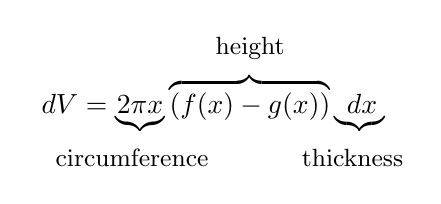
\begin{tikzpicture}
    \node at (0,0) {
      $\d V = \underbrace{2\pi x} \overbrace{(f(x)- g(x))}\underbrace{\d x}$
    };
    \node at (-1,-.7) {\small{circumference}};
    \node at (.5,.7) {\small{height}};
    \node at (1.8,-.7) {\small{thickness}};
  \end{tikzpicture}
\end{image}
Integrating $\d V$ will give us our desired volume.

%% What is the volume of such a shell?  Consider the shell at $x$.
%% Imagine that we cut the shell vertically in one place and ``unroll''
%% it into a thin, flat sheet. This sheet will be $f(x)-g(x)$ tall, and
%% $2\pi x$ wide since this is the circumference of the shell before it
%% was unrolled.  We may now write the integral


%% \begin{image}
%%   \begin{tikzpicture}
%%     \begin{axis}[
%%           xmin =0,xmax=4,ymax=5,ymin=-5,
%%           axis lines=none, xlabel=$x$, ylabel=$y$,
%%           every axis y label/.style={at=(current axis.above origin),anchor=south},
%%           every axis x label/.style={at=(current axis.right of origin),anchor=west},
%%           axis on top,
%%           width=5in,
%%           xtick={0,6}, xticklabels={$0$, $20$},
%%           ytick={0,3},yticklabels={$0$,$20$},
%%             clip=false,
%%       ]

            
%%       %\addplot [draw=penColor, thick] plot coordinates {(-3,-3) (0,0)};
%%       %\addplot [draw=penColor, thick] plot coordinates {(6,0) (0,0)};
%%       %\addplot [draw=penColor, thick] plot coordinates {(1.5,3) (3,-3)};
%%       %\addplot [draw=penColor, thick] plot coordinates {(1.5,3) (0,0)};

%%       %% slab
%%       \addplot [draw=penColor, fill=fillp,very thick] plot coordinates {(3,2) (1,2) (0,1) (2, 1) (3,2)};
%%       \addplot [draw=penColor, fill=fillp,very thick] plot coordinates {(0,.8) (0,1) (2,1) (2, .8) (0,.8)};
%%       \addplot [draw=penColor, fill=fillp,very thick] plot coordinates {(2,1) (2, .8) (3,1.8) (3,2) (2,1)};

%%       %\addplot [draw=penColor, fill=fillp,very thick] plot coordinates {(3,1.8) (1,1.8) (0,.8) (2, .8) (3,1.8)};
%%       %\addplot [draw=penColor, fill=fillp,very thick] plot coordinates {(3,2) (1,2) (0,1) (2, 1) (3,2)};



%%       \draw[decoration={brace,mirror,raise=.1cm},decorate,thin] (axis cs:0,.8)--(axis cs:2,.8);
%%       \draw[decoration={brace,mirror,raise=.1cm},decorate,thin] (axis cs:2,.8)--(axis cs:3,1.8);
%%       \draw[decoration={brace,raise=.1cm},decorate,thin] (axis cs:3,2.05)--(axis cs:3,1.75);
      
%%      % \addplot [->] plot coordinates {(0,0) (-4,-4)};
%%       %\node[anchor=north east] at (axis cs:-4,-4) {$z$};

%%       \node at (axis cs:3.15,1.9) {$\d x$};
%%       \node at (axis cs:2.8,0.8) {$f(x)-g(x)$};
%%       \node at (axis cs:1,.4) {$2x\pi$};       
%%     \end{axis}
%%   \end{tikzpicture}
%% \end{image}

\section{Shells around the axes}\index{shells}


Let's start by actually doing our motivating example above.


\begin{example}
  Consider the region below bounded by $f(x)=x+1$ and $g(x)=(x-1)^2$:
\begin{image}
\begin{tikzpicture}
  \begin{axis}[
      xmin=0, xmax=3,domain=0:3,
      clip=false,
      axis lines =center, xlabel=$x$, ylabel=$y$,
      every axis y label/.style={at=(current axis.above origin),anchor=south},
      every axis x label/.style={at=(current axis.right of origin),anchor=west},
      axis on top,
    ]
    \addplot [draw=none,fill=fillp] {x+1}\closedcycle;
    \addplot [draw=none,fill=white] {(x-1)^2}\closedcycle;
    \addplot [penColor,very thick] {x+1};
    \addplot [penColor2,very thick] {(x-1)^2};

    \node at (axis cs:2,3.3) [penColor] {$f$};
    \node at (axis cs:2.5,1.7) [penColor2] {$g$};
  \end{axis}
\end{tikzpicture}
\end{image}
  Find the volume of the solid of revolution formed by rotating this
  region around the $y$-axis.
  \begin{explanation}
    We'll solve this problem using accumulated shells. If we draw our shell, we see
    \begin{image}
\begin{tikzpicture}
  \begin{axis}[
      xmin=-3, xmax=3,domain=0:3,
      clip=false,
      width=4in,
      height=2in,
      axis lines =center, xlabel=$x$, ylabel=$y$,
      every axis y label/.style={at=(current axis.above origin),anchor=south},
      every axis x label/.style={at=(current axis.right of origin),anchor=west},
      axis on top,
    ] 
   

    \addplot [draw=none,fill=fillp!50!white] plot coordinates {(1.5,2.5) (1.5,.25) (-1.5,.25) (-1.5,2.5)};
    
    \draw[penColor,very thick,fill=fillp] (axis cs:0,2.5) ellipse (150 and 20);
    \draw[penColor,very thick,fill=white] (axis cs:0,2.5) ellipse (120 and 10);


   \draw[penColor, very thick, dashed, fill=fillp!50!white] (axis cs:0,0.25) ellipse (150 and 20);
   \draw[penColor, very thick, dashed,fill=white] (axis cs:0,0.25) ellipse (120 and 10);


     \addplot [penColor,very thick,domain=-3:0] {-x+1};
   \addplot [penColor2,very thick,domain=-3:0] {(-x-1)^2};
   
   \addplot [penColor,very thick] {x+1};
   \addplot [penColor2,very thick] {(x-1)^2};

    \node at (axis cs:2,3.3) [penColor] {$f$};
    \node at (axis cs:2.5,1.7) [penColor2] {$g$};

    
    \node at (axis cs:1.35,3) {$\d x$};
    \draw[decoration={brace,raise=.1cm},decorate,thin] (axis cs:1.2,2.6)--(axis cs:1.5,2.6);
    
    \addplot [very thick, penColor4] plot coordinates {(1.5,2.5) (1.5,.25)};
    \addplot [very thick, penColor4] plot coordinates {(-1.5,2.5) (-1.5,.25)};
    \addplot [very thick, penColor4, dashed] plot coordinates {(1.2,2.5) (1.2,.25)};
    \addplot [very thick, penColor4, dashed] plot coordinates {(-1.2,2.5) (-1.2,.25)};
    \draw[very thick, penColor]   (axis cs: -1.5,.25) arc(180:360:150 and 20);
  \end{axis}
\end{tikzpicture}
%% \caption{A plot of $f(x) = x+1$ and $g(x) = (x-1)^2$ with the
%%   ``shell'' indicated.}
%% \label{figure:shellIndicated}
    \end{image}
    Since the volume of each shell is
    \[
    \d V = 2\pi x (f(x) -g(x) ) \d x
    \]
    we may write 
    \begin{align*}
      \int_{\answer[given]{0}}^{\answer[given]{3}} 2\pi x(f(x)-g(x))\d x &= \int_{\answer[given]{0}}^{\answer[given]{3}} 2\pi x(\answer[given]{x+1}-(x-1)^2)\d x\\
      &= \eval{\answer[given]{2\pi x^3 -\frac{\pi x^4}{2}}}_{\answer[given]{0}}^{\answer[given]{3}}\\
      &=\answer[given]{\frac{27\pi}{2}}.
    \end{align*}
  \end{explanation}
\end{example}


Comparing our work above to our earlier work, we see that using shells
not only solves the problem with just one integral, we see that the
integral itself is somewhat easier than those in the previous
calculation! Things are not always so neat, but it is often the case
that one of the two methods will be simpler than the other, so it is
worth considering both methods.


\begin{example} 
Suppose the area bounded by $y=\sqrt{x}$, the line $y = 2x-1$, and the
$x$-axis is rotated around the $x$-axis,
\begin{image}
\begin{tikzpicture}
  \begin{axis}[
      xmin=0, xmax=1.2,ymax = 1.7, ymin = -.5,domain=0:1.2,
      clip=true,
      axis lines =center, xlabel=$x$, ylabel=$y$,
      every axis y label/.style={at=(current axis.above origin),anchor=south},
      every axis x label/.style={at=(current axis.right of origin),anchor=west},
      axis on top,
    ] 
  \addplot [draw=none,fill=fillp, domain=0:1] {sqrt(x)}\closedcycle;
    \addplot [penColor,very thick, samples = 100,smooth] {sqrt(x)};
    \addplot [penColor2,very thick,domain=0.5:1.5] {2*x-1};
     \addplot [draw=none,fill=white,very thick,domain=0.5:1] {2*x-1.02}\closedcycle;
  \end{axis}
\end{tikzpicture}
\end{image}
find the volume of this solid.
\begin{explanation}
While we could use accumulated cross-sections to compute this volume,
it would require \textit{two} integrals, (the industrious young
mathematician is encouraged to attempt to solve this problem using
accumulated cross-sections). However, here we will use the method of
shells. Let's see a picture:
\begin{image}
\begin{tikzpicture}
  \begin{axis}[
      xmin=0, xmax=1.2,ymax = 1.7, ymin = -1.7,
      clip=true,
      axis lines =center, xlabel=$x$, ylabel=$y$,
      every axis y label/.style={at=(current axis.above origin),anchor=south},
      every axis x label/.style={at=(current axis.right of origin),anchor=west},
      axis on top,
    ] 

    \addplot [draw=none, fill=fill1!50!white] plot coordinates {(.8,.6) (.36,.6) (.36,-.6) (.8,-.6)};
    
    \draw[penColor,dashed,very thick,fill=fillp!50!white] (axis cs:.36,0) ellipse (7 and 60);
    \draw[penColor,dashed,very thick,fill=white] (axis cs:.36,0) ellipse (5 and 50);
    
    \addplot [very thick, penColor4] plot coordinates {(.8,.6) (.36,.6)};
    \addplot [very thick, penColor4] plot coordinates {(.8,-.6) (.36,-.6)};
    \addplot [very thick, penColor4, dashed] plot coordinates {(.8,.5) (.36,.5)};
    \addplot [very thick, penColor4, dashed] plot coordinates {(.8,-.5) (.36,-.5)};

    \addplot [penColor,very thick, samples = 100,smooth,domain=0:1.2] {sqrt(x)};
    \addplot [penColor2,very thick,domain=0.5:1.5] {2*x-1};
    \addplot [penColor,very thick, samples = 100,smooth,domain=0:1.2] {-sqrt(x)};
    \addplot [penColor2,very thick,domain=0.5:1.5,domain=.5:1.2] {-2*x+1};

    \draw[penColor,very thick,fill=fillp] (axis cs:.8,0) ellipse (7 and 60);
    \draw[penColor,very thick,fill=white] (axis cs:.8,0) ellipse (5 and 50);

    \draw[decoration={brace,raise=.1cm},decorate,thin] (axis cs:.85,.65)--(axis cs:.85,.45);
    \node at (axis cs:.92,.55) {$\d y$};
    \draw[very thick, penColor]   (axis cs: .36,.6) arc(90:270:7 and 60);
  \end{axis}
\end{tikzpicture}
\end{image}
In this case, the volume of each shell is
\begin{image}
  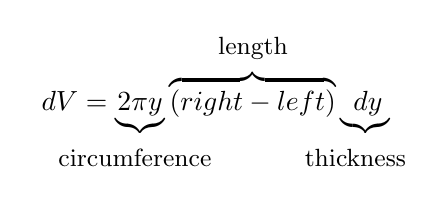
\begin{tikzpicture}
    \node at (0,0) {
      $\d V = \underbrace{2\pi y} \overbrace{(\text{right}-\text{left})}\underbrace{\d y}$
    };
    \node at (-1,-.7) {\small{circumference}};
    \node at (.5,.7) {\small{length}};
    \node at (1.8,-.7) {\small{thickness}};
  \end{tikzpicture}
\end{image}
Since we are integrating with respect to $y$, we have
\[
y=\sqrt{x} \qquad\Rightarrow\qquad x = \answer[given]{y^2}
\]
and
\[
y = 2x-1  \qquad\Rightarrow\qquad x= \answer[given]{\frac{y+1}{2}}.
\]
Hence the volume of our shell is
\[
\d V = 2\pi y \left(\answer[given]{\frac{y+1}{2} -y^2}\right) \d y
\]
Thus the the total volume of our solid of revolution is given by
\begin{align*}
  \text{Volume} &= \int_{\answer[given]{0}}^{\answer[given]{1}} \answer[given]{2\pi y (\frac{y+1}{2} - y^2)} \d y\\
  &= 2\pi\int_{\answer[given]{0}}^{\answer[given]{1}} \frac{y^2}{2}+\frac{y}{2} - y^3 \d y\\
  &= 2\pi\eval{\answer[given]{\frac{y^3}{6}+\frac{y^2}{4} - \frac{y^4}{4}}}_{\answer[given]{0}}^{\answer[given]{1}}\\
  &= \answer[given]{\frac{\pi}{3}}.
\end{align*}
\end{explanation}
\end{example}









\section{Shells around other lines}


What if we had wanted to rotate the region from the last example about
the line $y = -1$ instead of the $x$-axis? In this case, we draw a
picture and work much the same way as before. Let's see an example. 

\begin{example}
Suppose the area bounded by $y=\sqrt{x}$, the line $y = 2x-1$, and the
$x$-axis is rotated around the line $y= -1$,
\begin{image}
\begin{tikzpicture}
  \begin{axis}[
      xmin=0, xmax=1.2,ymax = 1.7, ymin = -.5,domain=0:1.2,
      clip=true,
      axis lines =center, xlabel=$x$, ylabel=$y$,
      every axis y label/.style={at=(current axis.above origin),anchor=south},
      every axis x label/.style={at=(current axis.right of origin),anchor=west},
      axis on top,
    ] 
  \addplot [draw=none,fill=fillp, domain=0:1] {sqrt(x)}\closedcycle;
    \addplot [penColor,very thick, samples = 100,smooth] {sqrt(x)};
    \addplot [penColor2,very thick,domain=0.5:1.5] {2*x-1};
     \addplot [draw=none,fill=white,very thick,domain=0.5:1] {2*x-1.02}\closedcycle;
  \end{axis}
\end{tikzpicture}
\end{image}
find the volume of this solid.  

\begin{explanation}
Let's see a picture:
\begin{image}
\begin{tikzpicture}
  \begin{axis}[
      xmin=0, xmax=1.2,ymax = 1.7, ymin = -3.7,
      clip=true,
      axis lines =center, xlabel=$x$, ylabel=$y$,
      every axis y label/.style={at=(current axis.above origin),anchor=south},
      every axis x label/.style={at=(current axis.right of origin),anchor=west},
      axis on top,
    ] 

    \addplot [draw=none, fill=fill1!50!white] plot coordinates {(.8,.6) (.36,.6) (.36,-2.6) (.8,-2.6)};
    
    \draw[penColor,dashed,very thick,fill=fillp!50!white] (axis cs:.36,-1) ellipse (7 and 160);
    \draw[penColor,dashed,very thick,fill=white] (axis cs:.36,-1) ellipse (5 and 150);
    
    \addplot [very thick, penColor4] plot coordinates {(.8,.6) (.36,.6)};
    \addplot [very thick, penColor4] plot coordinates {(.8,-2.6) (.36,-2.6)};
    \addplot [very thick, penColor4, dashed] plot coordinates {(.8,.5) (.36,.5)};
    \addplot [very thick, penColor4, dashed] plot coordinates {(.8,-2.5) (.36,-2.5)};

    \addplot [penColor,very thick, samples = 100,smooth,domain=0:1.2] {sqrt(x)};
    \addplot [penColor2,very thick,domain=0.5:1.5] {2*x-1};
    \addplot [penColor,very thick, samples = 100,smooth,domain=0:1.2] {-sqrt(x)-2};
    \addplot [penColor2,very thick,domain=0.5:1.5,domain=.5:1.2] {-2*x+1-2};

    \draw[penColor,very thick,fill=fillp] (axis cs:.8,-1) ellipse (7 and 160);
    \draw[penColor,very thick,fill=white] (axis cs:.8,-1) ellipse (5 and 150);

    \draw[decoration={brace,raise=.1cm},decorate,thin] (axis cs:.85,.65)--(axis cs:.85,.45);
    \node at (axis cs:.92,.55) {$\d y$};
    \draw[very thick, penColor]   (axis cs: .36,.6) arc(90:270:7 and 160);
  \end{axis}
\end{tikzpicture}
\end{image}
%% In this case, the volume of each shell is
%% \begin{image}
%%   \begin{tikzpicture}
%%     \node at (0,0) {
%%       $\d V = \underbrace{2\pi ???} \overbrace{(\text{right}-\text{left})}\underbrace{\d y}$
%%     };
%%     \node at (-1,-.7) {\small{circumference}};
%%     \node at (.5,.7) {\small{length}};
%%     \node at (1.8,-.7) {\small{thickness}};
%%   \end{tikzpicture}
%% \end{image}
Since we are integrating with respect to $y$, we have
\[
y=\sqrt{x} \qquad\Rightarrow\qquad x = \answer[given]{y^2}
\]
and
\[
y = 2x-1  \qquad\Rightarrow\qquad x= \answer[given]{\frac{y+1}{2}}.
\]
\begin{hint}
  The radius is now $y+1$, so the circumference is $2\pi(y+1)$
\end{hint}
Our cylindrical shells have the same width and height as in the
previous problem, but the circumference would changes, as the radius
is $\answer[given]{y+1}$.  Hence the volume of our shell is
\[
\d V = 2\pi (y+1) \left(\answer[given]{\frac{y+1}{2} -y^2}\right) \d y
\]
Thus the the total volume of our solid of revolution is given by
\begin{align*}
  \text{Volume} &= \int_{\answer[given]{0}}^{\answer[given]{1}} \answer[given]{2\pi (y+1) (\frac{y+1}{2} - y^2)} \d y\\
  &= 2\pi\int_{\answer[given]{0}}^{\answer[given]{1}} \frac{1}{2} + y - \frac{y^2}{2} -y^3 \d y\\
  &= 2\pi\eval{\answer[given]{\frac{y}{2}+\frac{y^2}{2}-\frac{y^3}{6} - \frac{y^4}{4}}}_{\answer[given]{0}}^{\answer[given]{1}}\\
  &= \answer[given]{\frac{7 \pi}{6}}.
\end{align*}
\end{explanation}


\end{example}


\end{document}
